\chapter{Du Christ à Jésus I}

\mn{X Gué le 14/02/23}


 \section{Eléments bibliographiques }

 \subsection{les apologistes}
 \begin{itemize}
     \item CLÉMENT D’ALEXANDRIE, Stromates I à V, Sources Chrétiennes, Paris.
     \item FÉDOU, M., La voie du Christ, Genèses de la christologie dans le contexte religieux de
l’Antiquité du IIe siècle au début du IVe siècle, Paris 2006.
     \item IRENÉE DE LYON, Contre les Hérésies. Dénonciation et réfutation de la prétendue gnose au
nom menteur, tr. par A. ROUSSEAU, Paris 19913.
     \item JUSTIN, OEuvres complètes, Paris 1994.
     \item ORIGENE, Traité des principes I, Sources Chrétiennes 252, Paris 1978.
     \item POUDERON, B., Les apologistes grecs du IIe siècle, Paris 2005.
     \item THEOPHILE D’ANTIOCHE, Trois livres à Autolycus, Sources Chrétiennes 20, Paris 1976.
 \end{itemize}

\subsection{les rationalistes}
\begin{itemize}
    \item B. COTTRET, Le Christ des Lumières. Jésus de Newton à Voltaire 1660-1760, Paris 1990.
    \item E. KANT, La religion dans les limites de la simple raison, Paris 2004
    \item X. TILLIETTE, La christologie idéaliste, Paris 1986.
\end{itemize}

% -------------------------------------------------------------------------------
\section{Introduction}


\paragraph{on ne part pas de Jésus historique} mais du Christ et du \textit{Logos}, titre universel. 
On présuppose que le partenaire du dialogue adhère à quelque chose de commun, le \textit{logos}.

\paragraph{Deux exemples dans l'histoire} Pour le dialogue, il faut un point commun. L'idée est plus grande que le concret historique, Jésus. Notre première approche a été de partir de l'histoire et de l'expérience. Ici, on va partir du spirituel et de l'universel. Au Ième siècle et XVIIIè.

\paragraph{faire de la christologie dans un monde pluraliste} Ce n'est pas facile d'entrer dans un autre type de culture.

% -------------------------------------------------------------------------------
\section{Dépasser le langage de la tribu}

Le premier dialogue a été entre les chrétiens juifs et les philosophes grecs. 

 \subsection{Paul à Athènes}

 \paragraph{Un des seuls récits de Paul avec des non-juifs} On ne voit pas trop de dialogues avec des non-juifs. Il reconnait la valeur de la recherche des Athéniens.
\begin{quote}
    
« Le Dieu qui a créé l’univers et tout ce qui s’y trouve (…) donne à tous la vie et le souffle, et
tout le reste (…). A partir d’une seul homme il a créé tous les peuples pour habiter toute la
surface de la terre, il a défini des temps fixes et tracé des limites de l’habitat des hommes ;
c’était pour qu’ils cherchent Dieu ; peut-être pourraient-ils le découvrir en tâtonnant, lui qui,
en réalité, n’est pas loin de chacun de nous car c’est en lui que nous avons la vie, le
mouvement et l’être, comme l’ont dit certains de vos poètes : ‘car nous sommes de sa race’ »
(Ac 17,24-28).
\end{quote}
 L'homme cherche Dieu en tâtonnant mais Dieu n'est pas loin de nous. \textit{colin maillard}. Dieu n'est pas inaccessible à l'homme car par la création, il est proche de tout homme. C'est différent de Rm 1. Le Paul de \textit{Luc} est plus \textit{optimiste} sur la nature humaine. 
 
\paragraph{Epiménide et Aratos} La premiere partie de Ac 17, 28 cite Epiménide et evoque la prière platonicienne. La deuxième partie (nous tirons...), le poête Aratos.
\begin{quote}
    
     il a voulu qu'ils cherchassent le Seigneur, et qu'ils s'efforçassent de le trouver en tâtonnant, bien qu'il ne soit pas loin de chacun de nous, 28car en lui nous avons la vie, le mouvement, et l'être. C'est ce qu'ont dit aussi quelques-uns de vos poètes: De lui nous sommes la race. Ac 17, 27-28
\end{quote}

\subsection{L’idée de Logos dans le NT}

 \paragraph{concentrée dans les écrits johanniques} 5 fois dans le prologue, Jn 1,1. et aussi une référence dans l'Apocalypse Ap 19,3 "Parole de Dieu". AUjourd'hui, on pense que le prologue viendrait d'un développement de la littérature sapientielle, et que le Logos serait la \textit{Sagesse} (Pr 8,22). Le \textit{Logos} participant à la Création.  Mais dans le prologue, une idée aussi d'accomplissement.


 

 
% -------------------------------------------------------------------------------
\section{L’importance de la christologie du logos au début du christianisme}

\paragraph{chez les intellectuels}

 \subsection{La convergence du christianisme et de la philosophie grecque}

 \paragraph{la philosophie grecque est une sagesse} Apprendre à vivre \textit{bien}. 

 \paragraph{les pères apologistes} se sont fait interprètes. Soucis de faire le pont, de dialoguer avec les autres. Recevoir des autres. En réaction avec la religiosité polythéiste, elle définit le Christ comme Logos. Si l'être du monde est apparu dans la figure de Jésus. "vous philosophe, parlez du logos, nous allons vous accompagner du logos tel que nous le connaissons".

 \paragraph{Logos stoicien} raison du monde, une entité bien connue : ce qui fait sortir le monde du chaos en harmonie. Le monde forme un tout cohérent, une unité. de plus, avec l'idée néo-platonicienne du logos, d'intermédiaire entre le \textit{un} et la \textit{multiplicité du monde}. Le Logos est l'émanation du un. Une virtualité de tous les êtres dans le \textit{logos}.

 \paragraph{Jésus est le logos venu dans le monde} donc:
 \begin{itemize}
     \item universel.     \item Lien avec Dieu.     \item Il se manifeste progressivement dans l'histoire. 
 \end{itemize}
 
\subsection{Le Logos un avec le Père, créateur et principe du monde}

 \paragraph{Idée du Logos, un avec Dieu} Théophile d'Antioche, Tatien, vont développer : Dieu est sage; donc il a une pensée, un logos. Et la parole, c'est le logos extériorisé. Au moment où il sort de Dieu, c'est la Création. 
 \begin{quote}
     Dieu dit et le monde est créé.
 \end{quote}

 Tatien : 


\begin{quote}
    « Dieu engendra son Logos, qui était immanent (endiatheton) en son sein, et le produisit avec
sa Sagesse avant toute chose. Il eut ce Logos comme ministre de toutes ses oeuvres, et par lui
tout a été fait. On l’appelle Principe, parce qu’il est le Principe et le maître de tout ce qui a été
créé par lui. C’est lui, Esprit de Dieu, Principe et Sagesse et Force du Très-Haut, qui
descendait sur les prophètes (…) » (Théophile d’Antioche, A Autolycus, II, 10)
\end{quote}


\begin{quote}
    « Avant que rien ne fût, [Dieu] tenait conseil avec [son Logos] lui qui est son intelligence et
son sentiment. Et quand Dieu décida de faire tout ce qu’il avait délibéré, il engendra son
Logos au-dehors (egennèsen prophorikon), premier-né de toute créature, sans être privé luimême
du Logos, mais ayant engendré le Logos et s’entretenant toujours avec son Logos. »
(Théophile d’Antioche, A Autolycus, II, 22)
\end{quote}

 
\begin{quote}
    « Nous ne disons donc pas, comme le pensent les hérétiques, qu’une partie de la substance de
Dieu se soit changée en fils ou que le Fils a été procrée par le Père à partir de rien, c’est-à-dire
en dehors de sa substance, de telle sorte qu’il fut un moment où il n’était pas, mais nous
disons, en supprimant toute signification corporelle, que la Parole et Sagesse est née du Père
invisible et incorporel, sans que rien ne se produise corporellement, comme la volonté
procède de l’intelligence… De même que jamais la lumière n’a pu exister sans son
rayonnement, de même le Fils ne peut être compris sans le Père (…) » (Origène, Traité des
principes, IV, 4, 1)
\end{quote}


\subsection{Universalité du Logos et le thème des «semences du Verbe»}

 \paragraph{Le thème du Logos disséminé : Justin et les autres} Justin, philosophe, converti au Christianisme, meurt martyr en 165 à Rome. Il n'a pas pensé sa conversion comme une rupture mais un accomplissement. 

Une apologie à l'empereur Antonin : 
\begin{quote}
    « Ceux qui ont vécu selon le Logos sont chrétiens, même s’ils ont été tenus pour athées,
comme par exemple, chez les Grecs, Socrate, Héraclite, et d’autres pareils, et, chez les
Barbares, Abraham, Ananias, Azarias, Misaël, Elie et quantité d’autres, dont nous renonçons
pour l’instant à énumérer les oeuvres et les noms (…). Dès lors aussi, ceux qui, parmi les
hommes des temps passés, ont vécu loin du Logos, furent mauvais, ennemis du Christ,
meurtriers de ceux qui vivaient selon le Logos, tandis que ceux qui ont vécu et qui vivent encore selon le Logos sont chrétiens, sans crainte et sans inquiétude » (Justin, \textit{Apologie}, 46,3-
4).
\end{quote}
\begin{Prop}
Pas besoin d'être chrétien pour accueillir le Verbe : Socrate,... sont des chrétiens.
Être Chrétien, c'est suivre la vérité, le \textit{Logos}.
\end{Prop}

\paragraph{Pour Celse, les Chrétiens sont des athées} car déclarent que les idôles sont des faux dieux. 


\paragraph{Toutes les paroles émanent du \textit{Logos}} idée stoicienne, christianisé en un visage, celui de Jésus. 

\paragraph{Influence stoïcienne et originalité chrétienne} 





\begin{quote}
    « Car la pluie de la grâce divine est déversée sur les justes et les injustes ; Dieu est-il le Dieu
des seuls juifs, et non aussi des gentils ? » (…) « Quand je dis : philosophie, je n’entends pas
celle du Portique, ou de Platon, ou d’Epicure, ou d’Aristote. Mais tout ce qui a été dit de bon
dans chacune de ces écoles, et qui nous enseigne la justice accompagnée de connaissance
religieuse, c’est cet ensemble que j’appelle philosophie. » (Clément d’Alexandrie, Stromates
V,3,18, 6-8)
\end{quote}


\subsection{Le Logos et l’histoire} Le problème de ces théologies, c'est de rester théorique. Comment rattacher à l'histoire, \textit{l'économie du Logos}. Dans son apologie, Justin vont se conformer au \textit{Logos tout entier}, le Christ. Clément d'Alexandrie pense l'économie à travers un très beau texte : 



\begin{quote}
    « Avant la venue du Seigneur la philosophie était indispensable aux grecs pour les conduire à
la justice ; maintenant elle devient utile pour les conduire à la vénération de Dieu. Elle sert de
formation préparatoire aux esprits qui veulent gagner leur foi par la démonstration (…). \textbf{Dieu
est la cause de toutes les bonnes choses}, des unes immédiatement et pour elles-mêmes,
comme de l’AT et du NT, des autres par corollaire, comme de la philosophie. Peut-être même
la philosophie a-t-elle été donnée elle aussi comme un bien direct aux Grecs, avant que le
Seigneur eût élargi son appel jusqu’à eux : car elle faisait leur éducation, tout comme la Loi
celle des juifs, pour aller au Christ. La philosophie est un travail préparatoire ; elle ouvre la
route à celui que le Christ rend ensuite parfait (…). Il n’y a, certes, qu’une route de la vérité,
mais elle est comme un fleuve intarissable, vers lequel débouchent les autres cours d’eau
venus d’une peu partout » (Clément d’Alexandrie, Stromates I, 5,1-3).
\end{quote}

\paragraph{hypothèse de la philosophie comme don de Dieu}
 La philosophie comme don du Dieu \textit{car elles faisaient leur éducation} : parallèle avec la Torah. La route de la vérité, c'est le Christ, grand fleuve, où se rejoignent d'autres courants. 

 Jacques Dupuis : la philosophie est une lampe.\sn{théologie du pluralisme}. Des théophanies dans le cas où elles sont des logophanies. \textit{L'ange du Seigneur à Mambré}, c'est le Logos.
 On voit Adam et le Christ avec Adam.

\begin{marginfigure}
    \centering

    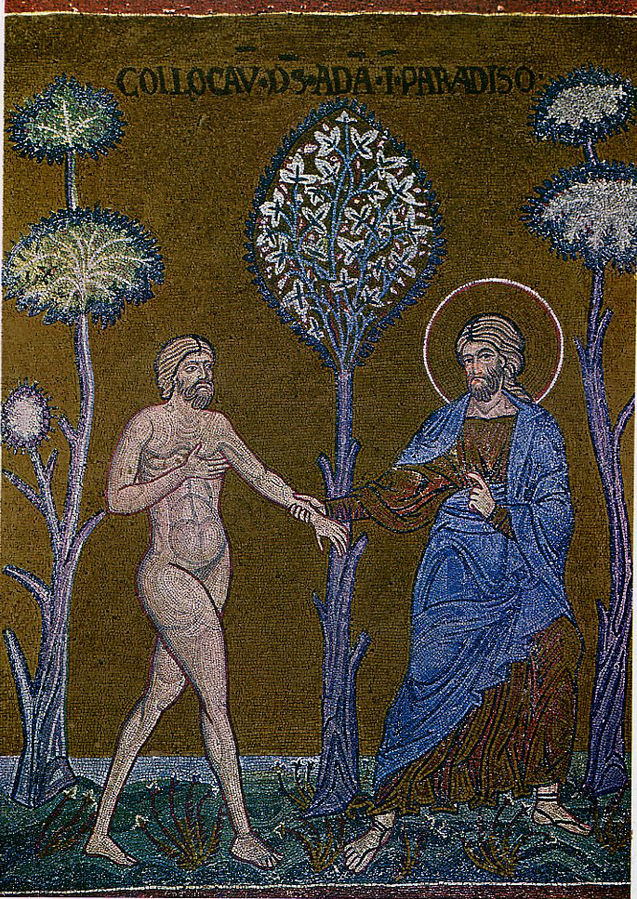
\includegraphics[width=\textwidth]{ChristologiePluraliste/Images/MonrealeAdam.jpg}
        \caption{le Christ et Adam.. Basilique de Monreale}
    \label{fig:my_label}
\end{marginfigure}


\paragraph{Mais alors le statut de la philosophie après Jésus-Christ}
 \begin{quote}
    « Si (…) la venue du Roi est annoncée par avance par les serviteurs que l’on envoie, c’est
pour la préparation de ceux qui auront à accueillir leur Seigneur. Mais lorsque le Roi est
arrivé, que ses sujets ont été remplis de la joie annoncée, qu’ils ont reçu de lui la liberté, qu’ils
ont bénéficié de sa vue, entendu ses paroles et joui de ses dons, alors du moins pour les gens
sensés, ne se pose plus la question de savoir ce que le Roi a apporté de nouveau par rapport à
ceux qui annoncèrent sa venue » (Irénée, Contre les hérésies VI, 34, 1).
\end{quote}


 
\subsection{L’identification problématique du Logos avec Jésus Christ} Ils se fondent sur l'histoire, sur le prologue. Et pourtant, le succès du Logos tend à mettre entre parenthèse le Jésus historique et son discours. Un peu trop philosophique.
Bernard Poudron, spécialiste des apologistes : 
 \begin{quote}
    La théologie « trinitaire » […] des apologistes est en réalité essentiellement une théologie du
Logos. Il est en effet remarquable que la plupart des apologistes ne mentionnent pas Jésus ou
le Christ en tant que personnage historique, mais n’évoquent le Fils qu’en tant qu’il est le
Logos de Dieu. » (Pouderon, Les apologistes, 91)
\end{quote}
Cela reste de l'ordre du principe philosophique. Risque de ne plus être lié au Jésus historique.



% -------------------------------------------------------------------------------
\section{ La christologie rationaliste dans un dialogue avec l’homme des Lumières}


 \subsection{Les Lumières : de la révélation historique à la révélation naturelle}

 \paragraph{Contexte de la modernité} Le magistère de la raison critique émerge de plus en plus. \textit{nouvelle religion}, le \textit{scientisme}, le \textit{positivisme} (Auguste Comte) :
 \begin{itemize}
     \item superstition
     \item Chrétien
     \item et aujourd'hui la science
 \end{itemize}
La science a remplacé pour certains la religion, qui allait nous libérer de beaucoup de choses.


\paragraph{comment présenter Jésus pour l'homme éclairé} A la suite des guerres de Religion, penser le vivre ensemble à partir d'un principe transcendant : les Lois de la nature sont plus stables que les vérités contestées de la révélation historique. \textit{Si vous tuez pour des vérités religieuses, du moins que la loi commune ne soit pas liée aux querelles de chapelle}
\paragraph{Deisme.} Dieu dans sa grande providence a organisé le monde avec la Loi Naturelle. Ce n'est plus le Logos. Et comment penser le Christ ? On va dire que le Christ a incarné la loi morale. Si, au deuxième siècle, on avait un dialogue cosmologique, ici on a un dialogue, un sous-jacent éthique.

\subsection{Le Christ comme le grand législateur} 

\paragraph{Christ comme grâce au Christ comme législateur} Bernard Cottret. Il monstre que Michelet, dans son \textit{histoire de la Révolution Française} a emprunté deux termes à la théologie : la \textit{grâce} et la \textit{la Loi}. L'ancien régime était marqué par la \textit{grâce} avec son caractère un peu arbitraire, avec la Révolution qui est de l'ordre de la \textit{Loi}. 

\paragraph{Vers la théologie de la Loi du XIXè} Or Cottret remarque que la théologie du XVIII est une théologie de la grâce, et en Angleterre avec John Locke, grand théologien anglais va donner de plus en plus l'image d'un monarque constitutionnel qui va aboutir à une théologie de la Loi. Le monarque constitutionnel se porte garant de la loi. 
Jésus est rétrogradé au rang de \textit{grand législateur} : Jésus n'est plus le Jésus qui fait des miracles, mais celui qui donne la loi, comme Moise, mais ici la loi naturelle. 

\paragraph{Grand inquisiteur de Dovstoievski} On arrête des gens parce qu'il fait des miracles : 
\begin{quote}
    je t'ai reconnu. prison. 
\end{quote}
Quand le miracle devient permanent, peut on encore parler de miracles ? Cela devient une loi.  \sn{Levinas et le Christ, et le risque d'être ordonné au monde ?}

On passe d'une prière d'intercession à une prière d'action de grâce. 

\paragraph{Morale naturelle concurrence la religion révélée} La religion et la morale naturelle plutot que la religion révélée.

 
\subsection{Le christianisme est aussi vieux que la création}

\paragraph{Universaliser le Christ ?} Il y a toujours des gens qui ont essayé d'universaliser le Christ. La Loi était présente depuis la Création du monde. Matthiew Tindal (1667,...), \textit{Le christianisme, aussi ancien que la Création, ou l'Evangile, répétition de la nature}. En bref, l'avènement du Christ n'annonce rien qui ne soit réellement nouveau. Il rappelle ce qui est depuis toujours. Bolingbroke (-1851) présente ainsi : 
 \begin{quote}
    « Le christianisme, tel que le présente l’évangile, contient un système religieux qui est non
seulement complet mais encore totalement dénué d’affectation. Il s’agit en réalité du système
de la religion naturelle qui aurait dû continuer sa course, pour le plus grand bien de
l’humanité, s’il avait été propagé avec la même simplicité que celle que le Christ avait utilisée
pour l’enseigner » (Bolingbroke, Philosophical Works, Genève 1968, t II, 322 cité par Cottret,
159).
\end{quote}
Affectation : tout ce que l'on a rajouté au dessus. 

\begin{quote}
« Jésus, comme Socrate, avait découvert la religion naturelle ; comme Socrate enfin, Jésus a
été trahi. Socrate et Jésus ne nous sont connus qu’au travers du témoignage suspect de Platon
et de saint Paul. (…) L’Église (…) constitue en fait une sorte d’écran entre le Christ et nous :
‘l’Evangile du Christ est une chose, l’Evangile de saint Paul, et de tous ceux qui se sont
greffés sur la même souche après lui, en est une autre’ (Bolingbroke, Philosophical Works,
Genève 1968, t II, 328 cité par Cottret 160). »
    
\end{quote}
Jésus a été trahi (on a mis de la religion dessus). Paul a trahi Jésus (sera repris par Harnack). 

\begin{quote}
«S’il y avait un système moral complet dans l’évangile, nous pourrions nous attendre à le
trouver dans les chapitres V, VI et VII de saint Matthieu \sn{sermon sur la montagne} dans la mesure où ils contiennent un
sermon prononcée par le Christ en personne et qui ne porte pas sur quelque point particulier
de doctrine, mais sur les devoirs de l’homme. Qu’y trouvons-nous ? De nombreux préceptes
moraux, sans doute excellents, mêlés de toutes sortes des considérations, provenant de
révélations personnelles, et pourtant conformes à ce que la loi de nature commande ou
prescrit, comme le démontre l’exemple des philosophes et des autres hommes de bien parmi
les païens » (Bolingbroke, Philosophical Works, Genève 1968, t II, 3 306-307 cité par Cottret
160).
    
\end{quote}
Ecarte la Croix 
\begin{quote}
« Quelle place laisser au mystère qui environne le crucifié ? Une certaine révolte se fait jour :
comment les chrétiens ont-ils pu parler au sujet de la mort de Jésus de sacrifice voulu par
Dieu ? » (Cottret, 161). « Imaginons un grand Prince qui gouvernerait un méchant peuple de
rebelles. Alors qu’il pourrait punir ses sujets, il choisit de leur pardonner. Mais il ordonne que
son Fils unique, son Fils bien-aimé, soit mis à mort pour expier leurs péchés et pour satisfaire
son royal courroux. Une telle action paraît-elle bonne, juste ou sage aux yeux de la raison ou à
la lumière de la nature, dénuée de tous préjugées ? » (Bolingbroke, Philosophical Works,
Genève 1968, t IV, 270-271 cité par Cottret 162).
    
\end{quote}


\paragraph{le Christ celui qui incarne la Loi voulue par Dieu}


\paragraph{Spinoza, XVII, mais dans la même lignée}

\begin{quote}
    C'est par lui que Dieu a fait connaitre l'enseignement moral qui constitue la religion universelle [\ldots] Jésus est philosophe. [\ldots] Il est l'idée de Dieu. [\ldots] Les philosophes peuvent être habités par le même esprit, l'éthique.
\end{quote}
Les philosophes n'ont pas besoin de la révélation historique du Christ. 

\subsection{Le Christ rationaliste d’E. Kant}
\paragraph{Kant}
1754-1804 La religion dans les limites de la simple raison.

 \paragraph{Le Christ, Archétype de l'homme agréable à Dieu} Idée pour Kant. L'idéal pour l'homme, c'est de faire la volonté de Dieu. Ce qui est important, ce n'est pas l'exemple mais l'idée. On n'a plus besoin de l'exemple quand on a compris. 
Incarnation : c'est une prise de conscience.


\begin{quote}

   « Nous élever à cet idéal de perfection morale c’est-à-dire à l’archétype de l’intention morale
dans toute sa pureté, voilà le devoir général de l’humanité et cette Idée même qui nous est
proposée comme modèle à atteindre par la raison, peut nous en donner la force. Or,
précisément parce que nous n’en sommes pas les auteurs et qu’elle a pris place en l’homme
sans que nous comprenions comment la nature humaine a seulement pu être susceptible de
l’accueillir, il vaut mieux dire : que cet archétype est descendu du ciel vers nous, qu’il a
revêtu l’humanité […]. » E. KANT, La religion dans les limites de la simple raison, Paris
2004, 134. 
\end{quote}
Kant ne parle jamais de Jésus mais du \textit{fils de Dieu} .


Quand on suit la morale Chrétienne, on est de bons chrétiens. Un biais moralisateur. 


\begin{quote}
« Si donc un tel homme, d’intentions vraiment divines, était à une certaine époque en quelque
sorte descendu du ciel sur la terre, donnant par sa doctrine, sa conduite, et ses souffrances
l’exemple d’un homme en soi agréable à Dieu, autant, bien entendu, qu’on peut le demander à
une expérience externe (l’archétype cependant d’un tel homme ne devant être recherché nulle
part ailleurs que dans notre raison), s’il avait par tout cela produit dans le monde un bien
moral immensément grand par le moyen d’une révolution dans le genre humain, il n’y aurait
pas lieu néanmoins de voir en lui autre chose qu’un homme engendré naturellement […]. » E.
KANT, La religion dans les limites de la simple raison, 137
    
\end{quote}

Et Strauss, influencé par Kant : 
\begin{quote}
« L’histoire de l’Évangile est au fond l’histoire de la nature humaine ramenée à une
conception idéale ; elle nous montre dans un individu ce que l’homme \textit{doit être}, ce qu’il peut
véritablement devenir en s’unissant à lui et en suivant sa doctrine et son exemple. » D. F.
STRAUSS, La vie de Jésus, Paris 1858, 692.
    
\end{quote}
\textit{du zollst}, l'impératif catégorique. 







% -------------------------------------------------------------------------------
\section{Conclusion}

Comment relier le Christ, le Logos avec la figure de Jésus : enjeu de la théologie contemporaine.


\begin{Synthesis}[théologie du logos]
    \begin{itemize}
        \item Non pas à partir de Jésus mais à partir du Christ universel, logos. Les pères apologistes avaient développé le \textit{logos} pour être intelligible pour les grecs. \textit{semence du verbe}
        \item difficulté de lier avec Jésus.
        \item pour les apologistes, le \textit{logos} par qui tout est créé plus que le fils de Marie.
        \item C'est un problème qu'on a avec une christologie ascendante ou descendante. Lien entre le particulier et l'universel. A reprendre à chaque génération.
    \end{itemize}
    
\end{Synthesis}

\begin{Synthesis}[Jésus législateur universelle]
    \begin{itemize}
        \item Rationel : un Christ qui incarne la loi morale. Ce n'est pas ce qui transgresse la loi (miracle,...), c'est le législateur universelle, c'est en ce sens qu'il est le sauveur
        \item articulation avec sa vie historique.
    \end{itemize}
\end{Synthesis}
 
















 